\setAuthor{Valter Kiisk}
\setRound{lõppvoor}
\setYear{2017}
\setNumber{G 3}
\setDifficulty{3}
\setTopic{Varia}

\prob{Laser}
Laserkiir ühtlase diameetriga $d=\SI{1}{mm}$ langeb risti kiilukujulise klaasplaadi esimesele pinnale (pindade vaheline nurk $\varphi=\ang{2}$). Laserkiire koosseisus on monokromaatsed komponendid lainepikkustega $\lambda_1=\SI{355}{nm}$ ja $\lambda_2=\SI{532}{nm}$. Klaasi murdumisnäitajad nendel lainepikkustel on vastavalt $n_1=\num{1.48}$ ja $n_2=\num{1.46}$. Leidke kaugus $l$ klaasplaadist, kus erineva lainepikkusega valguskiired on teineteisest täielikult eraldunud.

\hint
Eri värvi komponendid on täielikult eraldunud juhul, kui plaadist väljuvate laserkiirte tsentrite vaheline kaugus distantsil $l$ saab võrdseks kiire diameetriga.

\solu
Eri värvi komponendid on täielikult eraldunud juhul, kui plaadist väljuvate laserkiirte tsentrite vaheline kaugus distantsil $l$ saab võrdseks kiire diameetriga (vt joonis). Vastavalt ülesande andmetele on kõik nurgad väikesed, nii et murdumisseaduses $n_\alpha\sin\alpha=n_\beta\sin\beta$ võib võtta $\sin\alpha\approx\alpha$ ja $\sin\beta\approx\beta$ (kus $\alpha$ ja $\beta$ mõõdetakse radiaanides). Järelikult seos nurkade vahel muutub lineaarseks: $n_\alpha\alpha\approx n_\beta\beta$. Tänu sellele ei oleks ka lõppvastuse leidmise seisukohalt oluline valguse täpne langemisnurk klaasplaadile (tingimusel, et see nurk on $\ll 1$). Antud ülesande juhul langeb valgus esimesele pinnale risti. Sel juhul langemisnurk teisele pinnale ($\alpha$) on võrdne nurgaga $\varphi$ ja murdumisnurk vastavalt $\beta=n\alpha=n\varphi$, kus $n$ on klaasi murdumisnäitaja. Komponentide suundade erinevus on vastavalt $\Delta\beta=\Delta n\varphi=(n_1-n_2)\varphi$. Kuna nurk $\Delta\beta$ on väike, siis kiirte tsentrite vaheline kaugus on $\Delta\beta l$, kui nad on kaugusel $l$ plaadi teisest pinnast. Et nad oleks täielikult eraldunud, peab kehtima
\[
l\Delta\beta=l(n_1-n_2)\varphi=d,
\]
kust saame
\[
l = \frac{d}{(n_1-n_2)\varphi} = \SI{1.4}{m}.
\]

\begin{center}
	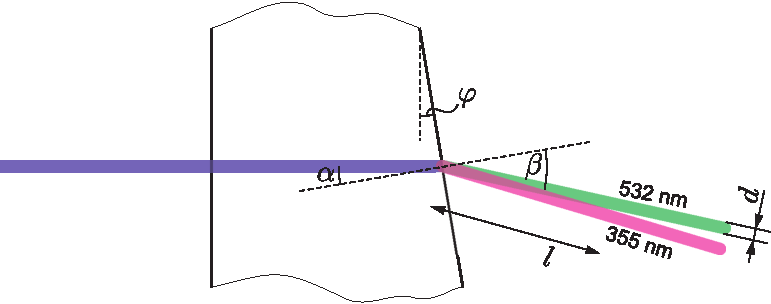
\includegraphics[width=0.93\linewidth]{2017-v3g-03-laser-lahend.pdf}
\end{center}

\probeng{Laser}
A laser beam with an even diameter $d=\SI{1}{mm}$ falls perpendicularly to the first surface of a wedge-shaped glass plate (the angle between the surfaces $\varphi=\ang{2}$). The laser beam consists of monochromatic components with wavelengths $\lambda_1=\SI{355}{nm}$ and $\lambda_2=\SI{532}{nm}$. The refractive indexes of the glass on these wavelengths are accordingly $n_1=\num{1.48}$ and $n_2=\num{1.46}$. Find the distance $l$ between the glass plate and the location where the light beams with different wavelength are completely separated from each other.

\hinteng
Components with different colors are completely separated if the distance between the centers of the laser rays leaving the plate at the distance $l$ becomes equal to the diameter of the rays.

\solueng
Different colored components are completely separated in the case where the distance between the centers of the laser rays exiting the plate gets equal to the diameters of the rays at a distance $l$ (see figure). According to the problem’s primary data all the angles are small so from the law of refraction $n_\alpha\sin\alpha=n_\beta\sin\beta$ we can take $\sin\alpha\approx\alpha$ and $\sin\beta\approx\beta$ (where $\alpha$ and $\beta$ are measured in radians). Therefore the relation between the angles starts to be linear: $n_\alpha\alpha\approx n_\beta\beta$. Thanks to this in terms of finding the final answer the exact falling angle of the light to the glass plate is not necessary (in the condition that this angle is $\ll 1$). In the given problem the light falls perpendicularly to the first surface. In this case the falling angle to the second surface ($\alpha$) is equal to the angle $\varphi$ and the angle of refraction is accordingly $\beta=n\alpha=n\varphi$ where $n$ is the refractive index of the glass. The difference of the directions of the components is accordingly $\Delta\beta=\Delta n\varphi=(n_1-n_2)\varphi$. Because the angle $\Delta\beta$ is small then the distance between the centers of the rays is $\Delta\beta l$ if they are at a distance $l$ from the plate’s second surface. For them to be completely separated the following must apply:
\[
l\Delta\beta=l(n_1-n_2)\varphi=d,
\]
from which we get
\[
l = \frac{d}{(n_1-n_2)\varphi} = \SI{1.4}{m}.
\]
\begin{center}
	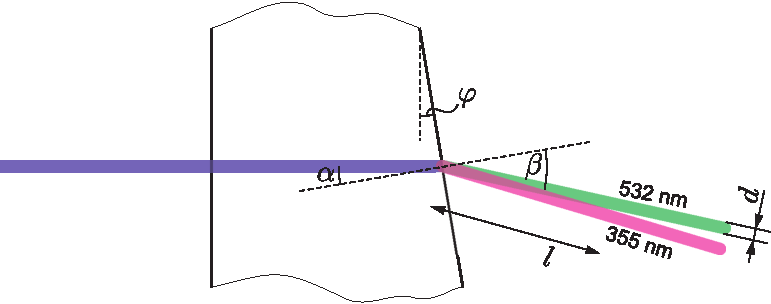
\includegraphics[width=0.93\linewidth]{2017-v3g-03-laser-lahend}
\end{center}
\probend